\chapter{Theoretical Background}

\section{Unstructured Data}

Unstructured data refers to information that does not follow a predefined schema or tabular format, making it inherently more complex to process and analyze than structured (typically stored in SQL databases) or semi-structured (typically managed by NoSQL databases) data. Examples include text documents, images, audio and video files, sensor logs, scientific data, and code, which vary widely in format, size, and origin and often require specialized techniques to extract meaningful insights.

\subsection{Embeddings}

Embeddings are numerical representations of data mapped into a continuous vector space (Figure~\ref{fig:data-1-a}), where semantically similar objects are placed close together (Figure~\ref{fig:data-1-b}). They bridge the gap between discrete, symbolic data and differentiable machine learning models, representing complex objects as fixed-length vectors. High-quality embeddings capture relevant features of the original data, supporting tasks such as classification, clustering, and similarity search \cite{Grohe-2020}.

\subsection{Distance Metrics}

Choosing an appropriate distance metric (Table~\ref{tab:distance-metrics}) ensures that embeddings accurately reflect the semantic similarity of the original unstructured data.

\begin{figure}[h]
    \centering
    \begin{subfigure}[t]{0.48\textwidth}
        \centering
        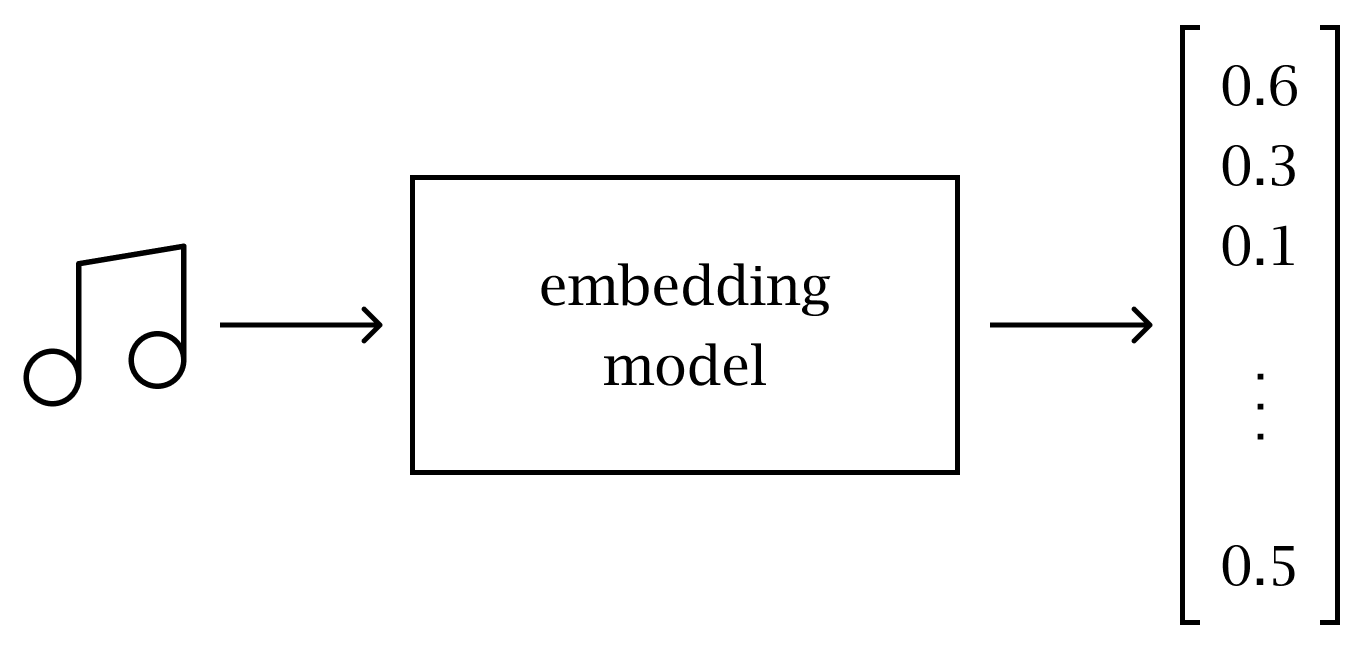
\includegraphics[width=\textwidth]{chapters/theory/data/figures/embedding.png}
        \caption{Unstructured data processed through a model to generate embeddings.}
        \label{fig:data-1-a}
    \end{subfigure}
    \hfill
    \begin{subfigure}[t]{0.48\textwidth}
        \centering
        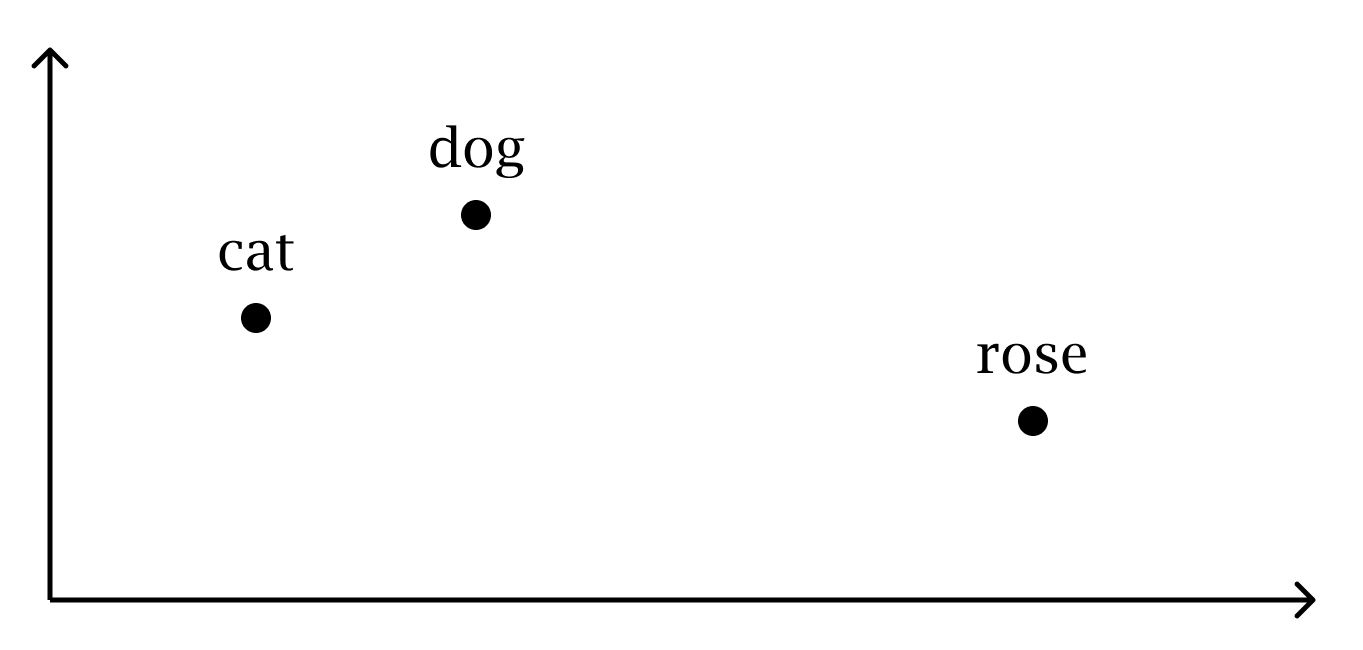
\includegraphics[width=\textwidth]{chapters/theory/data/figures/similarity.png}
        \caption{Semantically similar objects appear close together, while dissimilar ones are farther apart.}
        \label{fig:data-1-b}
    \end{subfigure}
    \caption{Illustration of the embedding process (a) and semantic similarity (b).}
    \label{fig:data-1}
\end{figure}

\begin{table}[h]
    \centering
    \renewcommand{\arraystretch}{2.3}
    \caption{Common similarity measures in vector databases.}
    \label{tab:distance-metrics}
    \begin{tabular}{|m{5cm}|m{8cm}|}
        \hline
        \textbf{Metric} & \textbf{Formula} \\ \hline
        $l_p$ (Minkowski) 
            & $\|x-y\|_p = \left(\sum_{i=1}^d |x_i-y_i|^p\right)^{1/p}$ \\ \hline
        $l_1$ (Manhattan) 
            & $\|x-y\|_1 = \sum_{i=1}^d |x_i-y_i|$ \\ \hline
        $l_2$ (Euclidean) 
            & $\|x-y\|_2 = \sqrt{\sum_{i=1}^d (x_i-y_i)^2}$ \\ \hline
        $l_\infty$ (Chebyshev) 
            & $\|x-y\|_\infty = \max_i |x_i-y_i|$ \\ \hline
        Cosine distance 
            & $d_{cos}(x,y) = 1 - (x \cdot y) / (\|x\|_2 \cdot \|y\|_2)
$ \\ \hline
        Dot (inner) product 
            & $s_{dot}(x,y) = \sum_{i=1}^d x_i \cdot y_i$ \\ \hline
        Hamming distance 
            & $d_{H}(x,y) = \sum_{i=1}^d 1(x_i \neq y_i)$ \\ \hline
    \end{tabular}
\end{table}
\section{Nearest Neighbor Search}

\subsection{Exact Nearest Neighbor Search}

\paragraph{Definition}

Given a set $P$ of points in a normed space $l_p^d$, preprocess $P$ so as to efficiently answer queries by returning a point $p \in P$ closest to a query point $q$.

This definition generalizes naturally to finding $k > 1$ nearest neighbors. In the $k$-NN search problem, $k$ points $p_1, \dots, p_k$ are returned such that each $p_i$ is the $i$-th closest point to $q$ \cite{Gionis-Indyk-Motwani-1999}.

\paragraph{Brute Force Approach}

The most straightforward approach for exact nearest neighbor search is the brute force (BF), or exhaustive search approach, which computes the distance between a query point and all points in the dataset to return the closest one. However, the computational cost of a single BF $k$-NN query using a chosen $l_p^d$ norm is $O(n \cdot d)$ \cite{Ukey-Yang-Li-Zhang-Hu-Zhang-2023}.

\paragraph{Structured Indexing Methods}

Several structured indexing methods have been proposed for exact $k$-NN search to efficiently handle low-dimensional datasets \cite{Ukey-Yang-Li-Zhang-Hu-Zhang-2023}:

\begin{itemize}
    \item \textbf{R-tree} and its variants (R*-tree, Hilbert R-tree, PR-tree): A height-balanced tree in which leaf nodes contain entries with an $n$-dimensional rectangle representing the bounding box of the associated spatial object, and non-leaf nodes contain entries that cover all rectangles in the entries of the lower node \cite{Guttman-1984}.
    \item \textbf{KD-tree}: A binary space-partitioning tree where each node stores a point from the dataset, and non-leaf nodes implicitly define a hyperplane that partitions the space into two child subtrees. At each level, the dimension with the largest spread is chosen, and the dataset is split at the median along that dimension \cite{Skrodzki-2019}.
    \item \textbf{Ball-tree}: A metric space-partitioning tree where each node defines a hypersphere containing a subset of the dataset. Each internal node is split in two steps: (1) the farthest point from the centroid of the points is selected as the first child centroid, and (2) the farthest point from this first centroid is selected as the second child centroid \cite{Dolatshah-Hadian-Minaei-2015}.
    \item \textbf{VP-tree} (and MVP-tree): A metric space-partitioning tree where each node selects a vantage point from its subset of points and partitions the points based on the median distance to this vantage point. Points closer than the median go to one child subtree, and points farther go to the other. This process is applied recursively, with distinct vantage points at each node, until leaf nodes containing a small number of points are reached \cite{Fu-Chan-Cheung-Moon-2000}.
\end{itemize}

\paragraph{Curse of Dimensionality}

As discussed above, these $k$-NN methods perform well in low-dimensional settings, but their efficiency degrades as the number of dimensions increases \cite{Ukey-Yang-Li-Zhang-Hu-Zhang-2023}.

The term \emph{curse of dimensionality} refers to the exponential growth of the volume of a space as the number of dimensions increases. This growth has significant implications for nearest neighbor search: as the dimensionality rises, data points become increasingly sparse. It causes distances between points to become increasingly similar, a phenomenon known as the \emph{concentration of measure}. As a result, the difference between the closest and farthest neighbors diminishes, reducing the effectiveness of standard distance metrics such as the $l_p^d$ norm.

Moreover, the impact of dimensionality depends on the relevance of the features: adding meaningful dimensions can improve contrast and preserve useful rankings of neighbors, while irrelevant dimensions reduce contrast and make distance-based queries less reliable \cite{Kouiroukidis-Evangelidis-2011}.

\subsection{Approximate Nearest Neighbor Search}

\paragraph{Definition}

Given a set $P$ of points in a normed space $l_p^d$, preprocess $P$ so as to efficiently answer queries by returning a point $p \in P$ for any given query point $q$, such that 
\[
d(p, q) \le (1 + \epsilon) \cdot d(q, P),
\]
where $d(q, P)$ is the distance from $q$ to its closest point in $P$.

This definition generalizes naturally to finding $k > 1$ approximate nearest neighbors. In the approximate $k$-NN search problem, $k$ points $p_1, \dots, p_k$ are returned such that the distance of $p_i$ to the query $q$ is at most $(1 + \epsilon)$ times the distance from the $i$-th nearest point to $q$ \cite{Gionis-Indyk-Motwani-1999}.

\paragraph{Motivation for Approximation}

In practical applications, the choice of features and distance metric is often heuristic, aiming to formalize what is fundamentally an intuitive notion of similarity. Consequently, insisting on exact nearest neighbors can be unnecessarily strict. Instead, determining an $\epsilon$-approximate nearest neighbor for a reasonable constant $\epsilon$ is usually sufficient for most purposes \cite{Indyk-Motwani-1998}.

Approximate nearest neighbor search aims to reduce the computational cost of similarity queries by relaxing the strict correctness requirement: the returned objects may not be the exact nearest neighbors. In practice, users often prefer faster responses that are sufficiently accurate rather than exact results, particularly in high-dimensional or large-scale datasets. The success of approximate methods relies on effectively balancing the trade-off between query efficiency and result quality \cite{Patella-Ciaccia-2009}.

\paragraph{Classification of Approximate Techniques}

Approximate nearest neighbor methods can be classified along several dimensions that reflect their applicability and design choices \cite{Patella-Ciaccia-2009}:

\begin{itemize}
    \item \textbf{Type of space} - Techniques can be specialized for different kinds of data spaces:
    \begin{itemize}
        \item Vector spaces with a specific $l_p^d$ distance.
        \item Vector spaces without restriction on the distance function.
        \item Metric spaces, where only the metric properties are assumed.
    \end{itemize}

    \item \textbf{Approximation mechanism} - How efficiency is achieved:
    \begin{itemize}
        \item Changing space: The search space is transformed or reduced (e.g., dimensionality reduction, bit approximations).
        \item Reducing comparisons: The search examines fewer candidates, either by
        \begin{itemize}
            \item aggressive pruning, or
            \item early stopping.
        \end{itemize}
    \end{itemize}

    \item \textbf{Quality guarantees} - Whether the method provides bounds on approximation errors:
    \begin{itemize}
        \item No guarantees: Heuristic approaches without formal bounds.
        \item Deterministic guarantees: Methods with provable maximum error bounds.
        \item Probabilistic guarantees: Techniques that guarantee correctness with a certain probability, either
        \begin{itemize}
            \item parametric, or
            \item non-parametric.
        \end{itemize}
    \end{itemize}

    \item \textbf{User interaction} - How parameters can be specified at query time:
    \begin{itemize}
        \item Static approach: Parameters are fixed at index construction; changing them requires rebuilding.
        \item Interactive approach: Users can adjust parameters dynamically at query time to trade off accuracy and efficiency.
    \end{itemize}
\end{itemize}

\begin{center}
    \vspace{0.5cm}
    *\hspace{2cm}*\hspace{2cm}*
    \vspace{0.3cm}
\end{center}

Unstructured data requires specialized representations to enable meaningful analysis. Embeddings map complex objects into a continuous vector space where semantic similarity can be quantified, while distance metrics determine how similarity is measured. Nearest neighbor search provides a framework for retrieving similar items, with exact methods offering precision and approximate methods trading some accuracy for efficiency. These concepts form the foundation for exploring specific algorithms for approximate nearest neighbor search, exemplified by hash-based, tree-based, and graph-based approaches.